% IEEE standard conference template; to be used with:
%   spconf.sty  - LaTeX style file, and
%   IEEEbib.bst - IEEE bibliography style file.
% --------------------------------------------------------------------------

\documentclass[letterpaper]{article}
\usepackage{spconf,amsmath,amssymb,graphicx}
\bibliographystyle{IEEEbib}

\usepackage{hyperref}
\hypersetup{
    colorlinks=true,
    linkcolor=blue,
    filecolor=magenta,      
    urlcolor=blue,
    pdftitle={Overleaf Example},
    pdfpagemode=FullScreen,
}
\usepackage{graphicx}
\usepackage{caption}
\usepackage{subcaption}
\usepackage{tikz}
\usepackage{dirtytalk}

\usepackage{cleveref}
\usepackage[english]{babel}

\usepackage{todonotes}

% Plotting Tex Stuff from https://pypi.org/project/tikzplotlib/
\usepackage{pgfplots}
\usepackage{float}
\DeclareUnicodeCharacter{2212}{−}
\usepgfplotslibrary{groupplots,dateplot}
\usetikzlibrary{patterns,shapes.arrows}
\pgfplotsset{compat=newest}
\usepackage{svg}

% CUSTOM STUFF TO REDUCE SPACING AT TITLES

% \usepackage[compact]{titlesec}
% \titlespacing{\section}{0pt}{2ex}{1ex}
% \titlespacing{\subsection}{0pt}{1ex}{0ex}
% \titlespacing{\subsubsection}{0pt}{0.5ex}{0ex}


% Example definitions.
% --------------------
% nice symbols for real and complex numbers
\newcommand{\R}[0]{\mathbb{R}}
\newcommand{\C}[0]{\mathbb{C}}

% bold paragraph titles
\newcommand{\mypar}[1]{{\bf #1.}}
\newcommand{\code}{\textit}

\newcommand{\grabenseifner}{\textit{Generalized Rabenseifner}}

% Title.
% ------
\title{Optimization of Distributed Sum of Outer Products (DSOP)}
%
% Single address.
% ---------------
\name{David Enderlin, Noé Heim, Roy Schubiger, Elwin Stephan, Patrick Ziegler} 
\address{Department of Computer Science\\ ETH Z\"urich\\Z\"urich, Switzerland}

% For example:
% ------------
%\address{School\\
%		 Department\\
%		 Address}
%
% Two addresses (uncomment and modify for two-address case).
% ----------------------------------------------------------
%\twoauthors
%  {A. Author-one, B. Author-two\sthanks{Thanks to XYZ agency for funding.}}
%		 {School A-B\\
%		 Department A-B\\
%		 Address A-B}
%  {C. Author-three, D. Author-four\sthanks{The fourth author performed the work
%		 while at ...}}
%		 {School C-D\\
%		 Department C-D\\
%		 Address C-D}
%

\begin{document}
%\ninept
%
\maketitle
%

\section{Abstract}
Computing the outer products of pairs of vectors, each pair stored on different nodes, and distributing their sum lies at the core of optimizing distributed deep learning. This paper proposes the \code{Generalized Rabenseifner} for distributed sum of outer products (DSOP), an algorithm that computes the DSOP using multiple participants. The proposed algorithm can be used to optimize distributed training of deep neural networks using a data-parallel approach by replacing the gradient averaging, typically using an \textit{allreduce}, with the proposed algorithm.
Compared to a baseline allreduce algorithm, our \grabenseifner{} algorithm achieves a median speedup of up to 3x.

\section{Introduction}\label{sec:intro}

Machine Learning is rapidly developing into an essential tool in modern systems. Deep Learning is a popular model used in modern machine learning systems. Optimizing the training of deep neural networks becomes an essential aspect as datasets become increasingly larger. A popular approach to accelerate training deep neural networks is using a data-parallel approach. This approach replicates the neural network across multiple computing nodes. The individual nodes can compute the forward and backward propagation steps independently. However, there needs to be a synchronization step to synchronize the gradients across the individual nodes. This synchronization step induces an allreduce operation. \cite{demystifying_hoefler}

Recent work by Bakker et al. showed that the gradient of feedforward and recurrent neural networks exhibit an outer product derivative structure in \cite{outer_product_structure_NN_derivatives}. This project aims to exploit this structure by studying the problem of the DSOP. Algorithms that solve the DSOP can then be used as a component to synchronize gradients across multiple nodes in distributed deep learning.

In the DSOP, there are $P$ hosts $p_1, ..., p_P$, each host $p_i$ having two vectors $a_i$, $b_i$. They engage in a computation such that all of the $P$ hosts end up with a local copy of the matrix $G$: % = \sum_{i = 1}^{P} a_i \cdot b_{i}^{\top}$.
\begin{equation}
    G = \sum_{i = 1}^{P} a_i \cdot b_{i}^{\top}
\end{equation}

This project aims to evaluate, design, and implement different efficient algorithms to compute $G$. First, we evaluate different implementations using procedures provided in MPI to compute the DSOP efficiently. Furthermore, we propose a novel algorithm to solve the DSOP, which optimizes bandwidth and performance. Moreover, we identify extensions to the proposed algorithm that can take the network heterogeneity into account and address the sparsity of inputs.
All source code and benchmarks results are publicly available on GitHub\footnote{\url{https://github.com/elwin/dphpc}}.

\section{Related Work}

Deep Learning has become an integral part of modern science. Improving the training time of deep neural networks has become increasingly important due to the growth of datasets, the complexity of problems they solve, and network sizes. Ben-nun and Hoefler provide a good overview of current and future parallelization strategies in \cite{demystifying_hoefler}.

The demand for distributed training of deep neural networks has led to various systems that leverage the message passing interface (MPI). For example, Horovod \cite{horovod} introduces an open-source library that uses ring reduction to enable distributed training in TensorFlow. Vishnu et al. \cite{distributed_TF_with_MPI} also propose a modification to TensorFlow to enable TensorFlow on clusters. In addition, there is a myriad of papers that try to apply MPI to distributed machine learning \cite{distributed_TF_with_MPI, ma2016theano_MPI, distributed_ML_for_computational_engineering_using_MPI}.

An approach for data-parallel training at scale is provided in Blink \cite{blink}, a collective communication library that tries to optimize communication in the face of hardware heterogeneity. A further approach is provided in Nguyen et al. \cite{topology_aware_sparse_allreduce}: The authors propose a sparse-ring-ring allreduce algorithm, which uses topology-aware and data compression techniques.


\section{Background}

One can group algorithms that compute the DSOP into two groups: allgather and allreduce, as illustrated in \Cref{fig:allgather_allreduce}. The most important collective operations in MPI used in these algorithms are allgather, broadcast, scatter, allreduce, and reduce-scatter. The following paragraphs describe the most important algorithms used in allgather and allreduce and present the cost model used to model our algorithms.

\begin{figure}[htp]
    \centering
    \begin{subfigure}{0.4\linewidth}
         \centering
         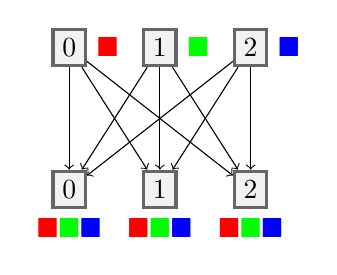
\begin{tikzpicture}[node distance=13mm and 7mm, square/.style={rectangle, draw=black!60, fill=black!5, very thick, minimum size=4mm}]
            %Nodes
            \node[square,label=below:$\color{red}\blacksquare\color{green}\blacksquare\color{blue}\blacksquare$] (b0)               {0};
            \node[square,label=below:$\color{red}\blacksquare\color{green}\blacksquare\color{blue}\blacksquare$] (b1) [right=of b0] {1};
            \node[square,label=below:$\color{red}\blacksquare\color{green}\blacksquare\color{blue}\blacksquare$] (b2) [right=of b1] {2};
            
            \node[square,label=right:$\color{red}\blacksquare$] (t0) [above=of b0]      {0};
            \node[square,label=right:$\color{green}\blacksquare$] (t1) [right=of t0]    {1};
            \node[square,label=right:$\color{blue}\blacksquare$] (t2) [right=of t1]     {2};
            
            %Lines
            \draw[->] (t0) -- (b0);
            \draw[->] (t0) -- (b1);
            \draw[->] (t0) -- (b2);
            
            \draw[->] (t1) -- (b0);
            \draw[->] (t1) -- (b1);
            \draw[->] (t1) -- (b2);
            
            \draw[->] (t2) -- (b0);
            \draw[->] (t2) -- (b1);
            \draw[->] (t2) -- (b2);
        \end{tikzpicture}
        \caption{Allgather}
        \label{fig:allgather}
     \end{subfigure}
     \;\;\;\;\;\;
     \begin{subfigure}{0.4\linewidth}
        \centering
         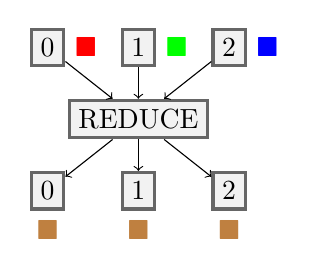
\begin{tikzpicture}[node distance=4mm and 7mm, square/.style={rectangle, draw=black!60, fill=black!5, very thick, minimum size=4mm}]
            %Nodes
            \node[square,label=right:$\color{red}\blacksquare$]     (t0)                {0};
            \node[square,label=right:$\color{green}\blacksquare$]   (t1) [right=of t0]  {1};
            \node[square,label=right:$\color{blue}\blacksquare$]    (t2) [right=of t1]  {2};
            
            \node[square] (aggregate) [below=of t1] {REDUCE};
            
            \node[square,label=below:$\color{brown}\blacksquare$] (b1) [below=of aggregate]   {1};
            \node[square,label=below:$\color{brown}\blacksquare$] (b0) [left=of b1]           {0};
            \node[square,label=below:$\color{brown}\blacksquare$] (b2) [right=of b1]          {2};
            
            %Lines
            \draw[->] (t0) -- (aggregate);
            \draw[->] (t1) -- (aggregate);
            \draw[->] (t2) -- (aggregate);
            
            \draw[->] (aggregate) -- (b0);
            \draw[->] (aggregate) -- (b1);
            \draw[->] (aggregate) -- (b2);
        \end{tikzpicture}
        \caption{Allreduce}
        \label{fig:allreduce}
     \end{subfigure}
     \caption{Illustration of the most commonly used collective operations.}
     \label{fig:allgather_allreduce}
\end{figure}

% \mbox{}\\[-45pt]

\subsection{Allgather and Allreduce}

Allgather represents an operation where each participating process contributes some data and receives the data contributed by all other processes. This notion of allgather suggests that an allgather algorithm that computes the DSOP contains a step where the data from all processes are distributed to every other process. The most important algorithms used for implementing allgather in Open MPI are Bruck \cite{Bruck:97}, recursive doubling, neighbor, and the ring algorithm. \cite{openMPI_decision_tree_4_0_2, openMPI_decision_tree_4_1_2,Chen:05}

Compared to allgather, the allreduce operation is composed of data movement and incorporates an operation executed on the data. The canonical operation fitting the setting of computing the DSOP is addition. The most important algorithms used to implement the allreduce operation in Open MPI are recursive doubling, the ring algorithm, and Rabenseifner's algorithm. \cite{openMPI_git, openMPI_decision_tree_4_0_2, openMPI_decision_tree_4_1_2, Rabenseifner:05}

Multiple algorithms are required to implement collective communication operations in MPI efficiently. Different algorithms provide different tradeoffs. Therefore, one has to decide on an algorithm based on the amount of data movement and the number of processes in the collective communication operation.
Open MPI uses a decision tree to select a suitable allreduce or allgather algorithm based on the total number of nodes, the size of the data, and, for allreduce, whether the reduction operation is commutative \cite{openMPI_decision_tree_4_0_2, openMPI_decision_tree_4_1_2}.
An extension to hierarchical networks introduces further complexity in choosing and designing such algorithms. \cite{improving_collective_operations_in_MPICH}

\subsection{Cost Model}

The cost model under which we evaluate our algorithms considers three dimensions: communication cost, the number of additions and multiplications per node. The network communication is modeled using the LogGP model. The addition and multiplication is indicated by the number of floating-point additions/multiplications performed in a node.
With these three entities, the cost model can capture the tradeoff that the individual approaches incur when computing the DSOP.

The LogGP model uses the following standard definitions to model the communication: latency $L$, host overhead $o$ for sending and receiving, the gap $g$ between messages, number of processes $P$, and the gap-per-byte $G$ (inverse of the bandwidth). We simplify the model by assuming that $g < o$. Furthermore, due to the problem at hand, the amount of data being transferred depends on the input sizes $N$ and $M$, and the algorithms used in the MPI-collective operations depend on the decision tree used in Open MPI 4.0.2, as can be seen in \cite{openMPI_decision_tree_4_0_2}.


\section{Implementation}

This section presents all algorithms we implemented that are relevant to the results. Other approaches that turned out to be less effective than the baseline were left out in the interest of brevity. We asymptotically model their costs alongside the algorithms using the previously described cost model.\\[-23pt]

\subsection{Basic Implementation}\label{sec:baseline}
As a first step, we present our baseline algorithms for solving the DSOP problem based on allgather and allreduce. 

In our basic \code{allgather} algorithm, all of the $P$ processes first distribute their two input vectors to all other processes using \verb|MPI_Allgather|. Then, after a process has received all vectors from the other nodes, it will compute the outer product $G_i = a_i \cdot b_{i}^{\top}$ for each received vector pair and sum up all the computed outer products to get the final matrix $G$. The cost for this baseline implementation using allgather can be modeled as follows:

\begin{tabular}{r l}
    Communication   &   $\mathcal{O}\left(P \cdot \left(o + L + (N + M) \cdot G \right)\right)$ \\
    Addition        &   $\mathcal{O}(P\cdot NM)$ \\
    Multiplication  &   $\mathcal{O}(P\cdot NM)$
\end{tabular}

The communication part is entirely determined by the \verb|MPI_Allgather| implementation. Here, we considered the neighbor exchange algorithm implemented in Open MPI as described in \cite{Chen:05}. Due to the chosen input parameters (vector size and the number of processes), this is the algorithm Open MPI selects for all allgather operations in our benchmarks. \cite{openMPI_decision_tree_4_0_2}

Our other baseline algorithm is based on an allreduce approach. All $P$ processes first calculate the outer product $G_i = a_i \cdot b_{i}^{\top}$ of their vector pair and then use a single \verb|MPI_Allreduce| to compute the sum of all matrices on all nodes.

The allreduce implementation used by Open MPI in all our benchmarks is a segmented ring allreduce. The chosen allreduce implementation is responsible for both the network cost and the cost of adding all intermediate matrices. The multiplications are due to the initial outer-product calculation. Here, another parameter $S$ is introduced, representing the number of elements in each segment. The segment size used by Open MPI is 1MB and thus $S = 2^{17}$. \cite{openMPI_decision_tree_4_0_2}

\begin{tabular}{r l}
    Communication   &   $\mathcal{O}\big(\frac{NM}{S}\left(L + o + S \cdot G \right)$ \\
                    &   $\; + \, P \left(L + o + \frac{NM}{P}\cdot G \right)\big)$ \\
    Addition        &   $\mathcal{O}(NM)$ \\
    Multiplication  &   $\mathcal{O}(NM)$
\end{tabular}

The cost models already show the main difference between the allgather and allreduce approach. An allgather approach performs more local computations while transferring fewer data over the network. In contrast, an allreduce approach trades fewer local computations for larger network transfers and more communication.\\[-23pt]

\subsection{Allreduce Ring} \label{allreduce-ring}
One of the better performing algorithms is the \code{allreduce-ring}. First, all of the $P$ processes compute the local outer product $G_i = a_i \cdot b_{i}^{\top}$ of their vectors, similar to the \code{allreduce} baseline, but instead of using the Open MPI implementation \verb|MPI_Allreduce|, the algorithm uses a custom reduction algorithm using a ring structure.

The algorithm divides the local matrix into $P$ chunks, and each process sends a different chunk to the next process in the ring. Each process then receives a chunk from the previous process, adds its matching chunk, and sends it to the next process. After $(P-1)$ rounds, each process possesses one chunk of the final result matrix. An allgather using the ring structure concludes the algorithm by each process sending the final chunk through the ring and forwarding any received chunks. This takes another $(P-1)$ steps, after which all processes possess the full final matrix $G$.

This is a reimplementation of the ring allreduce algorithm in Open MPI. We present it here because it performs better than using \verb|MPI_Allreduce| for the allreduce operation in most cases. We discuss this in \Cref{Discussion}.

\begin{tabular}{r l}
    Communication   &   $\mathcal{O}\big(P \left(o + L + \frac{NM}{P}\cdot G \right)\big)$ \\
    Addition        &   $\mathcal{O}(NM)$ \\
    Multiplication  &   $\mathcal{O}(NM)$
\end{tabular}

The communication cost is only asymptotic, but in reality, there is a constant factor of $2$ because the algorithm performs the $(P - 1)$ rounds twice, once for calculating a chunk for the final matrix and once for exchanging those final chunks.

\subsection{Generalized Rabenseifner for DSOP}\label{sec:grabenseifner}
The Open MPI \code{allreduce-rabenseifner} algorithm is a combination of a reduce-scatter implemented with recursive vector halving and recursive distance doubling, followed by an allgather implemented with recursive doubling (butterfly). \cite{Rabenseifner:05}

This algorithm is the basis for the proposed algorithm we call the \grabenseifner{}. \textit{Rabenseifner's} first butterfly is replaced with an allgather round to distribute all vectors to each process.
Then, each process calculates its local chunk of the final matrix, namely a continuous region of the final matrix stored in row-major order.
This partitioning can be achieved by partitioning the rows into contiguous rows and assigning them to individual processes.
Then, using an \verb|MPI_Allgather|, all the final chunks are distributed, such that in the end, each process has a local copy of the complete final matrix $G$.

\begin{tabular}{r l}
    Communication   &   $\mathcal{O}\big(P \cdot \left(o + L + (N+M) \cdot G \right)$ \\
                    &   $\; + \, P \cdot \left(o + L + \frac{NM}{P} \cdot G \right) \big)$ \\
    Addition        &   $\mathcal{O}(NM)$ \\    % (P-1) \frac{NM}{P} 
    Multiplication  &   $\mathcal{O}(NM)$ % P * NM/P = NM
\end{tabular}

The communication cost of the \grabenseifner{} is based on the underlying allgather implementation by Open MPI, which uses the neighbor exchange algorithm for our experimental configurations. The \grabenseifner{} algorithm performs two allgather operations, once with $N + M$ elements to exchange all vector pairs and once with $\frac{NM}{P}$ elements, the number of elements in the process' chunk of the final matrix. The addition and multiplication costs are from performing one outer product for the process' chunk for each vector pair, resulting in $P\cdot \frac{NM}{P} = NM$ additions and multiplications.

\subsection{Further Approaches}

% TODO review Roy, Dave, Noé

In the process of refining the previously mentioned approaches, we implemented several other algorithms as part of the evaluation process. The corresponding results are less relevant, as they do not perform as well.

\code{allgather-async} and \code{bruck-async} were attempts to take existing allgather algorithms for exchanging the vector pairs and perform outer product computations while some data was still in flight using non-blocking send and receive operations.

The \code{allreduce-butterfly} is a simple reimplementation of \code{allreduce} using a butterfly structure to send the data around. The matching implementation is similar to the \code{recursive-doubling} algorithm of Open MPI.

Similar to pipelining inside allgather, we tried to pipeline the \code{allreduce-butterfly} and the allreduce ring algorithm to perform the reduction step (matrix addition) while data was in flight. We also pipelined the first allgather step in the \grabenseifner{} to perform the outer product computations in parallel with the data transfers. All these attempts showed at most marginal improvements in runtime since the majority of the runtime can be attributed to communication, so we do not gain much when cutting down on calculation time. Nonetheless, there is still more room for pipelining as we did not pipeline all that was possible (see \Cref{sec:future_work}).


\section{Experimental Results}

\subsection{Benchmark Setup}
% How we measure, what we measure, why we measure it the way we do

All benchmarks were run on the Euler III cluster with a varying number of physical nodes. Each node contains a quad-core Intel Xeon E3-1585Lv5 processor, clocked between 3.0 and 3.7 GHz and 32GB of DDR4 memory, clocked at 2133 MHz. The cluster is arranged as a two-layer fat tree: 45 nodes are connected together via a 10G ethernet switch in a single bay; 27 of such bays are connected via 4x40G ethernet switches to one of Euler's core switches. Even though each node contains 4 cores, for our benchmarks, only 1 process runs per node.

All our code is compiled using gcc version 9.3.0 with the flags \texttt{-O3 -std=c++17 -mavx -mavx2 -mfma} and Open MPI 4.0.2. Note that the Rabenseifner algorithm is not present in the decision tree of this particular version of Open MPI, it has only been added in version 4.1 \cite{openMPI_git, openMPI_decision_tree_4_0_2, openMPI_decision_tree_4_1_2}.

The experiments are run on multiple input configurations. An input configuration is composed of the sizes $N$, $M$ of the input vectors $a_i$ and $b_i$ respectively, and the number of processes $P$. The experiments are restricted to the following ranges of parameter values:\\[-17pt]
% N = M & \in \{1000, 2000, 3000, 4000, 5000, 6000, 7000, 8000\} \\
\begin{align*}
N = M & \in \{1000\cdot i \ \ |\ \ 1 \leq i \leq 8,\ i \in \mathbb{N}\} \\
P & \in \{8, 16, 32, 48\} \\[-18pt]
\end{align*}
The range for the number of processes $P$ is mainly motivated by the limited access to the cluster, as students can only request up to 48 nodes at a time. Furthermore, the range of the input sizes $N$, $M$ is limited by the provided memory, since for larger matrices, the jobs run into memory limits. Moreover, the constraint that our experiments only consider $N = M$ is driven by limiting the number of configurations our experiments explore. Limiting the number of configurations enabled us to do more repeated measurements and, therefore, increased the results' repeatability. Finally, it has to be noted that all algorithms work independently of $N$ and $M$. However, for the experiments at hand, the algorithms were optimized for the case where $N = M$, i.e., for square matrices. But all the algorithms can easily be generalized for arbitrary values for $N$, $M$.

Each configuration is repeated 25 times with the same node assignment, meaning that each MPI process runs the algorithm 25 times.
Before each iteration, all processes are synchronized using \verb|MPI_Barrier|.
The results of the first iteration is discarded as a warm-up iteration.
The remaining iterations are aggregated into a single observation by only looking at the median of these measurements within one node assignment.

Different jobs have potentially different node assignments, possibly leading to varying performance results across otherwise identical input parameters. Therefore, each job is scheduled between 109 and 150 times to get a distribution over observations. To avoid confusion, we will call each of these jobs a \say{repetition} while each of the 25 repetitions within the same job is an \say{iteration}. Hence, for any given set of input parameters, we have at least 109 observations. Due to long queueing times for jobs with many nodes, the jobs running on 32 or 48 nodes tend to have fewer repetitions, while the ones with 8 and 16 nodes all have 150.

Runtimes are measured as differences in the timestamp returned by \verb|MPI_Wtime|.
The runtime for a process is measured from when the \verb|MPI_Barrier| call returns to the point where the process has completed its participation in the algorithm.
This point is after the process has the final matrix but may include additional data transfers to other processes that are still part of the algorithm.
After the experiment is finished, it results in one runtime value per process; the runtime for the experiment is the maximum of these values.


The evaluation considers statistics based on percentiles as we look at a distribution of observations. However, due to the variability in measurements and non-normally distributed observations, the statistics are estimated using a nonparametric 95\% confidence interval, which uses the same method to the \textit{percentile confidence interval} using bootstrap, as used in \cite[Chapter 5.7]{modern_applied_statistics_with_S}.

\begin{figure}[bhtp!]
    \centering
    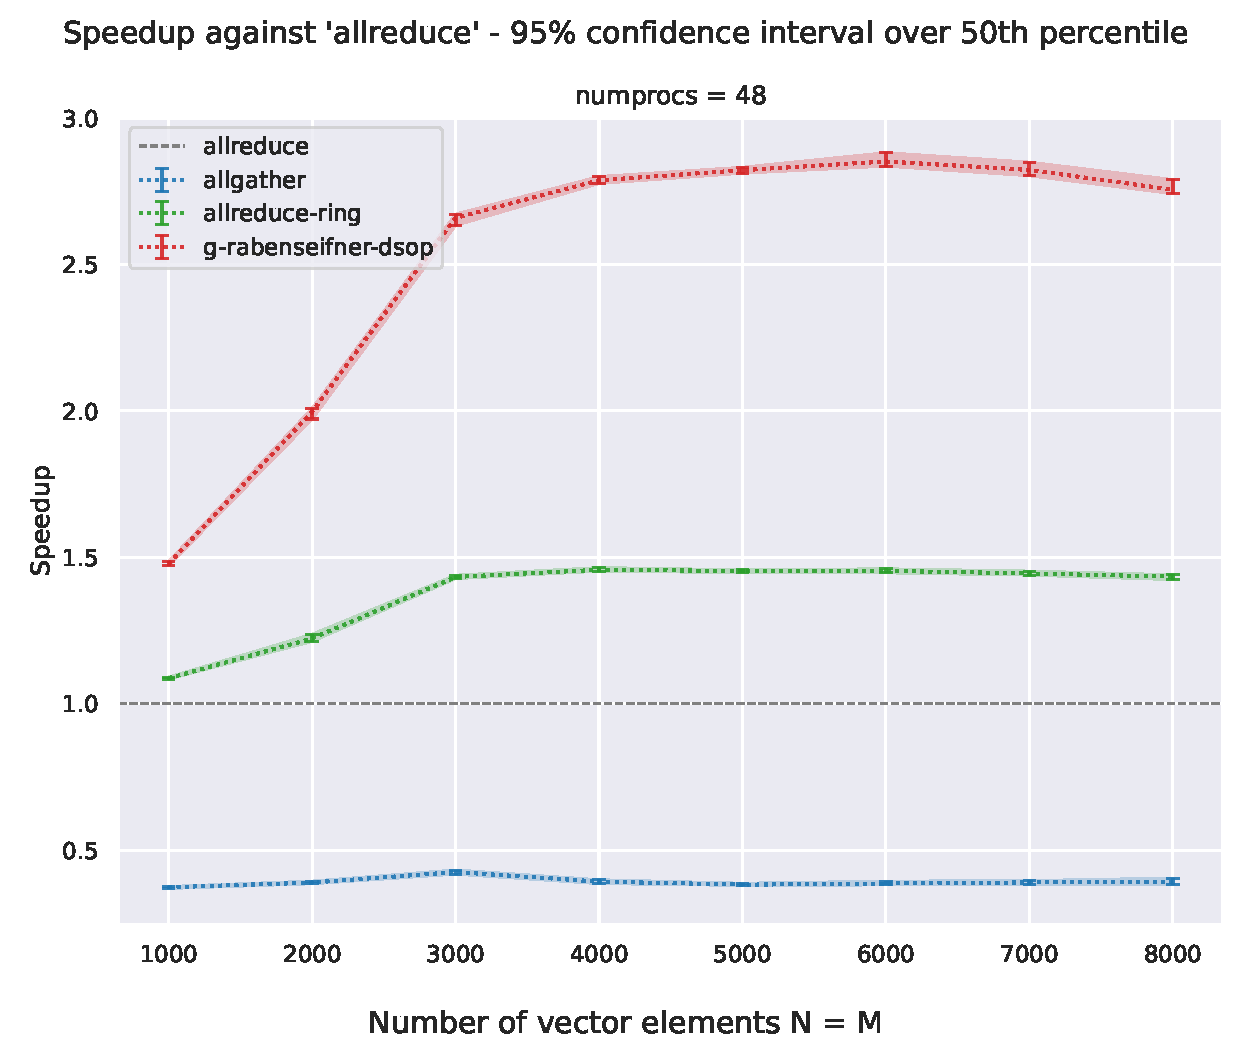
\includegraphics[width=0.95\columnwidth]{plots/speedup_plot_N_numprocs_48__baseline_allreduce_percentile_50_CI_0.95_with_errorbar.pdf}
    \caption{Median speedup against base allreduce implementation with 95\% confidence interval, run with 48 nodes}
    \label{fig:speedup-48-50-95}
\end{figure}


\subsection{Results}
    
Here, we present the key results from our experiments.
For the sake of brevity, we only show selected plots.
More plots can be found in the appendix in \nameref{app:figs} as well as in the GitHub repository linked in \Cref{sec:intro}.

\begin{figure}[htp]
    \centering
    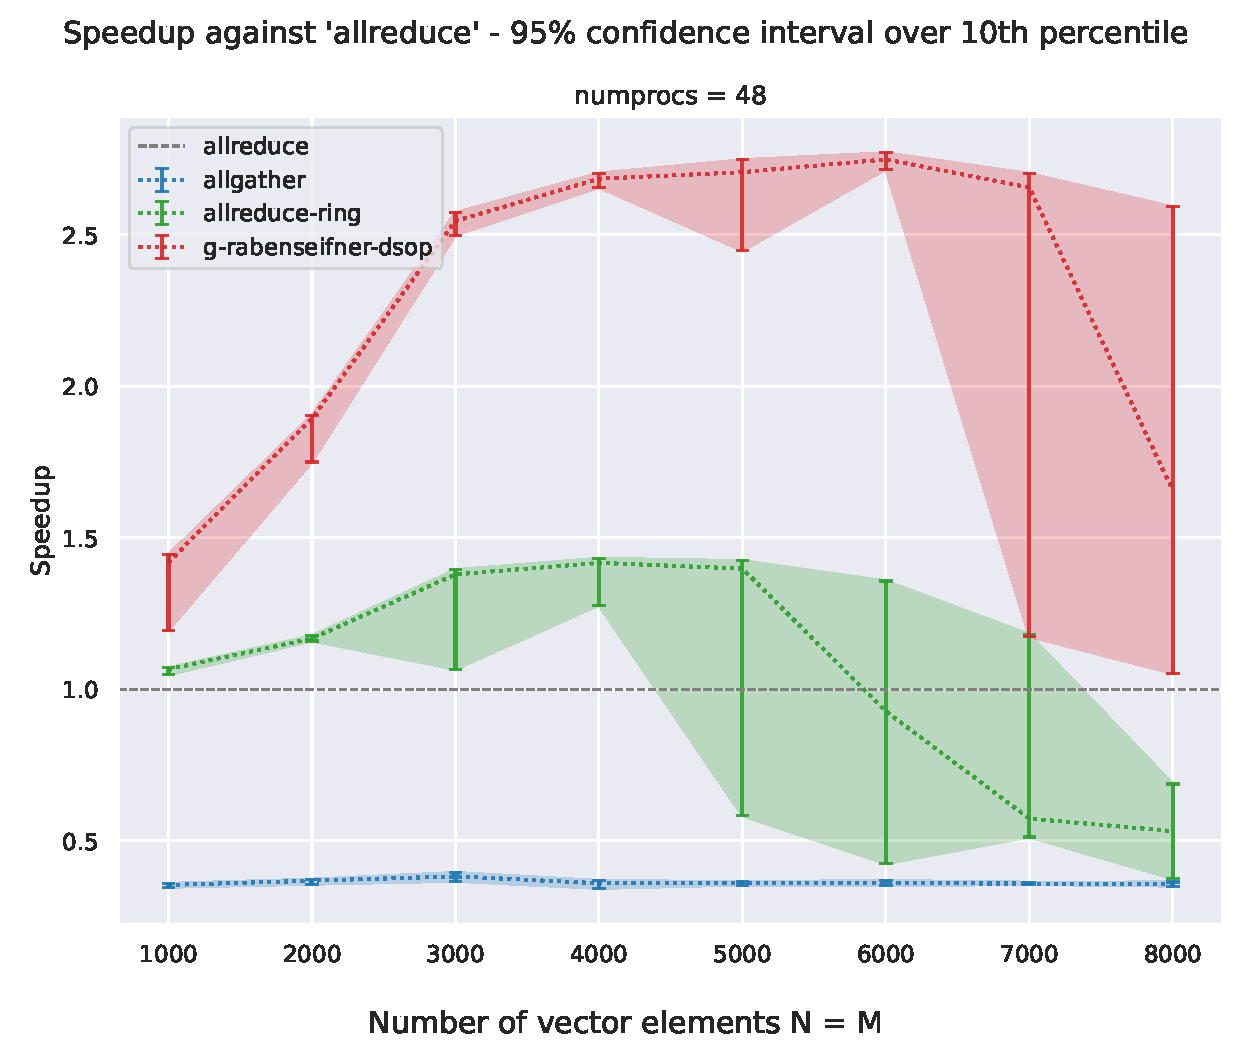
\includegraphics[width=0.95\columnwidth]{plots/speedup_plot_N_numprocs_48__baseline_allreduce_percentile_10_CI_0.95_with_errorbar.pdf}
    \caption{10th percentile of speedups against base allreduce implementation with 95\% confidence interval, 48 nodes}
    \label{fig:speedup-48-10-95}
\end{figure}

\begin{figure}[htp]
    \centering
    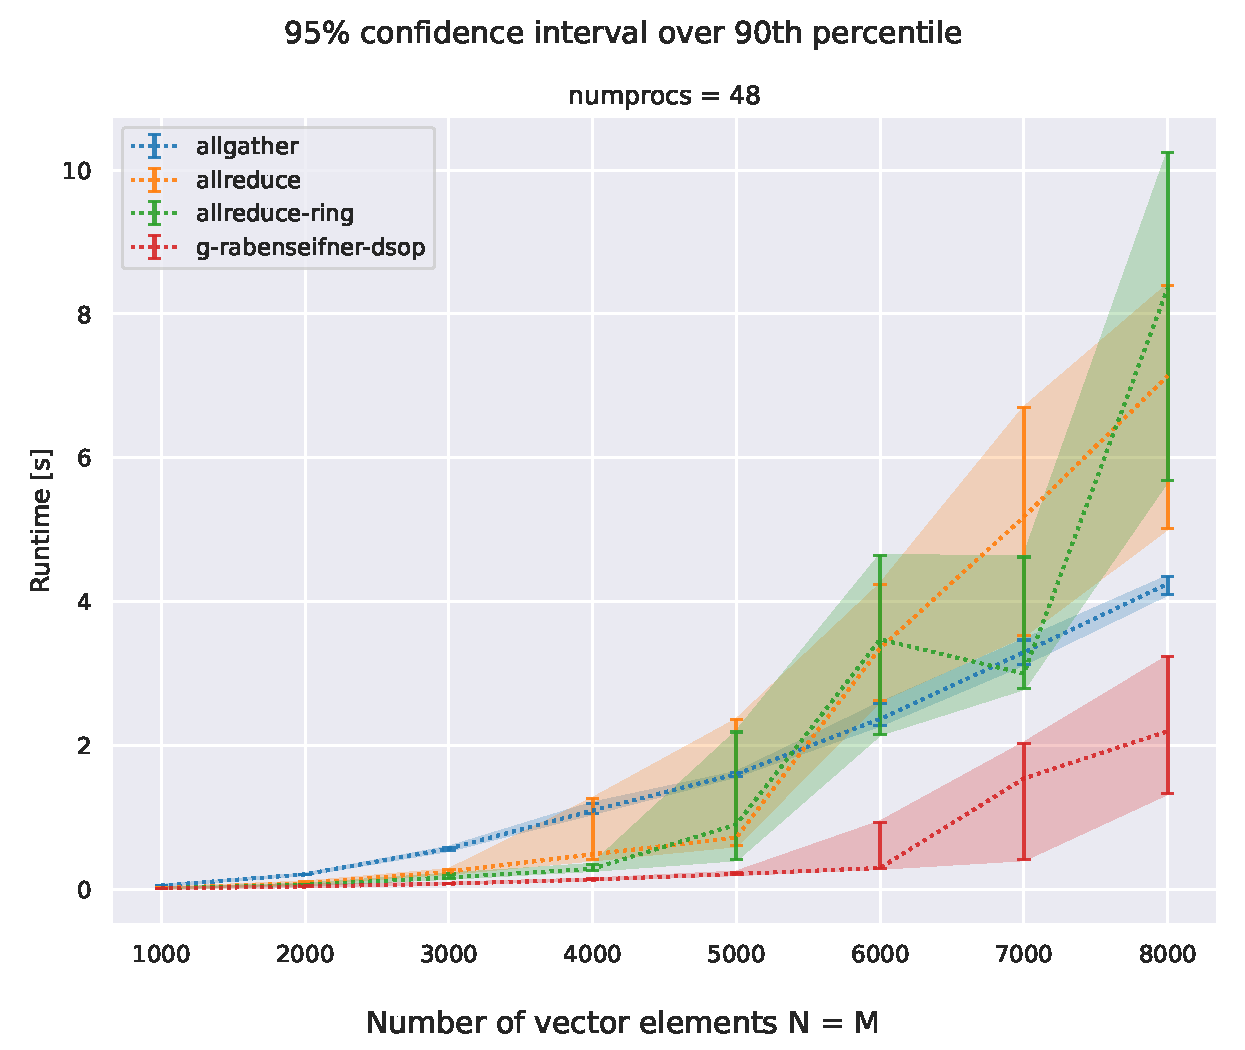
\includegraphics[width=0.95\columnwidth]{plots/runtime_numprocs_48_N_percentile_90_CI_0.95_with_errorbar.pdf}
    \caption{90th percentile of runtimes with 95\% confidence interval, run with 48 nodes}
    \label{fig:runtime-48-90-95}
\end{figure}

In the plot legends, \textit{allreduce} and \textit{allgather} refers to the two baseline algorithms described in \Cref{sec:baseline}.
The label \textit{allreduce-ring} refers to our allreduce ring algorithm from \Cref{allreduce-ring} and \textit{g-rabenseifner-dsop} refers to the \grabenseifner{}.
\Cref{fig:speedup-48-50-95} shows the median speedup of the benchmarked implementations against the baseline allreduce implementation with a 95\% bootstrap confidence interval.
In \Cref{fig:speedup-48-10-95}, we see the same speedup plot, but for the 10th percentile. For each observation, the speedup is calculated, giving us a distribution of speedups over all repetitions.
% The bootstrap confidence interval for the selected percentile is computed over this distribution for the corresponding percentile statistic.



In \Cref{fig:runtime-48-90-95}, we see the absolute runtime for the same experiment. This graph shows the 95\% bootstrap confidence interval around the 90th percentile of observations, meaning that 90\% of the jobs had a faster runtime than indicated by the dotted lines.



Because runtimes can vary between observations, we also present the distributions of runtimes over observations as violins in \Cref{fig:runtime-violin-48-log}. The violins show all observed values and the boxplots (without the central box) inside the violins show the 95th and 5th percentile as horizontal lines and the median as a slightly longer line. Because the violins for the \grabenseifner{} algorithm are quite bottom-heavy, the median line often overlaps the 5th percentile line at the bottom of the violin.

\begin{figure}[t]
    \centering
    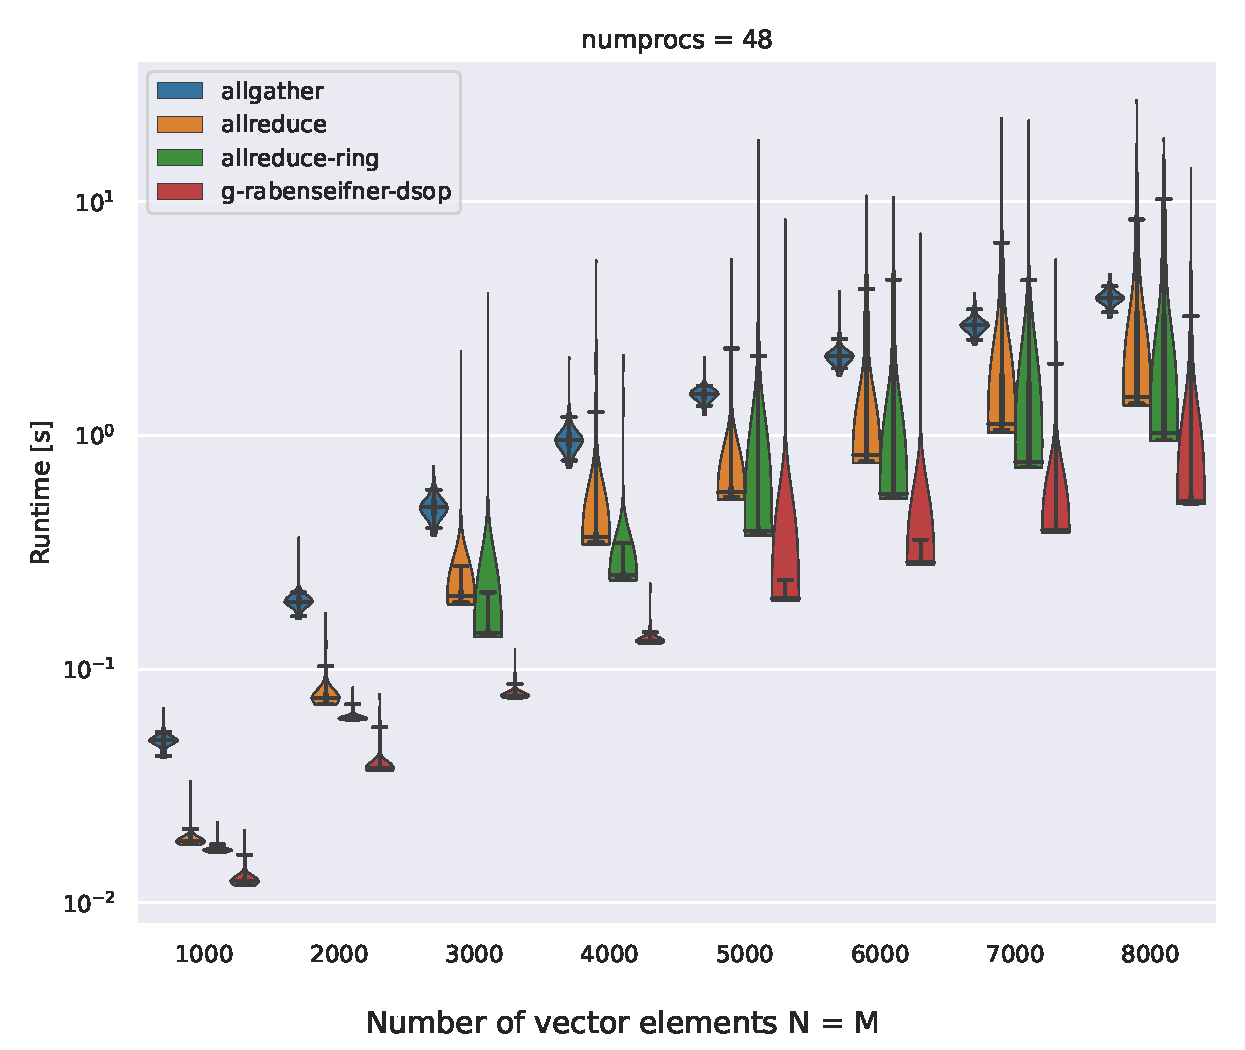
\includegraphics[width=0.95\columnwidth]{plots/cmp_numprocs_48_log_scale.pdf}
    \caption{Runtime distributions per implementation on 48 nodes.}
    \label{fig:runtime-violin-48-log}
\end{figure}

\section{Discussion}\label{Discussion}

In \Cref{fig:speedup-48-50-95}, we see a more than 2.5x median speedup of the \grabenseifner{} algorithm compared to the allreduce baseline. Even considering the 10th percentile of speedups in \Cref{fig:speedup-48-10-95}, meaning 90\% of observed speedups were higher, shows a clear advantage except for \\ $N \in \lbrace 7000, 8000 \rbrace$. Therefore, our algorithm still outperforms existing algorithms in a near worst-case scenario with reasonable certainty.

Additionally, the improvement of our algorithm compared to the existing methods is confirmed by comparing the 90th percentile of speedups to the allreduce baseline. This shows for 16, 32, and 48 processes, the speedup is larger than 3x in most cases (plots not shown). It even reaches values between 6x and 14x for a few cases. Therefore, the proposed algorithm outperforms the existing methods by a large margin in a best-case scenario.

In general, the experiments show a higher variability for larger inputs, especially for $N \in \lbrace 7000, 8000 \rbrace$. This variability can be attributed to network congestion from other jobs running on the cluster and the effect of node assignment. The relative location of nodes corresponding to a job seems to have a much bigger effect on runtimes when larger amounts of data are sent over the network.

The same behavior can be observed in \Cref{fig:runtime-violin-48-log}. The spread of runtimes increases, starting at $N=5000$, with outliers over an order of magnitude slower than the median. Furthermore, the plot suggests that the \grabenseifner{} sends fewer data over the network than the two allreduce implementations because they start showing a large spread in runtimes at $N=3000$.

All plots also include measurements for the implementations \code{allgather} and \code{allreduce-ring}.
The \code{allgather} implementation is the other of our two baseline implementations.
In the median case, the \code{allgather} is inferior to all other shown algorithms due to the large amount of local computation, which is performed redundantly at every node.
However, because the algorithm only requires small data transfers, the overall runtime performance is stable across all experiments and outperforms allreduce on 16 nodes or fewer.

The \code{allreduce-ring}, which just reimplements the allreduce ring algorithm used in Open MPI, surprisingly, outperforms the allreduce baseline in many cases. However, the speedup advantage is not as clear cut as with the generalized Rabenseifner because the 95\% confidence intervals do overlap the allreduce baseline in the worst-case scenarios in \Cref{fig:speedup-48-10-95,fig:runtime-48-90-95}. Nevertheless, there is a significant median speedup as seen in \Cref{fig:speedup-48-50-95}. We suspect this improvement over the allreduce-baseline may be due to compiler optimizations. Our code is compiled with AVX, AVX2, and FMAs enabled, while Open MPI has none of these enabled. Furthermore, in our \code{allreduce-ring} implementation, the outer-product step and the allreduce step are implemented in the same function, which could help the compiler better optimize the whole implementation. Because the allreduce runtime is dominated by the send and receive operations, these differences in local computations should not impact the total runtime to this extent. Further investigation is needed to find the root cause of these differences.


\section{Future Work}\label{sec:future_work}

While the \grabenseifner{} already provided excellent results, combining the proposed solution with further approaches can lead to additional improvements.

% \subsection{Topology Awareness}

Topology awareness has huge potential to reduce the total runtime of the algorithm. The proposed \grabenseifner{} can easily be extended to multiple variants using subgroups. In these variants, one can optimize the communication by using topology-aware information. An instantiation of such a variant is motivated by the approach proposed by Gong et al. in \cite{network_performance_aware_collective_communication_operations_in_the_cloud}. One can adapt their network performance aware operations to the \grabenseifner{} by instantiating a network hierarchy as proposed in \cite{network_performance_aware_collective_communication_operations_in_the_cloud} to perform the allreduce operation.
% A first, naive version towards such a variant has been tried with a subgroup-variation of the \grabenseifner{}. This subgroup-variant introduces redundant computation by partitioning the final matrix only within the given subgroup. However, more sophisticated approaches need to be evaluated to improve the performance.

% \subsection{Sparsity}

The resulting outer products will also be sparse when working with sparse vectors. Therefore, one can expect substantial performance improvements by optimizing the amount of data sent over the network for sparse input vectors, as most of the runtime arises from communication and not calculation. In \cite{narang2017exploring}, the authors are pruning RNNs to get a sparse network which could then be combined with an algorithm that exploits this sparsity during DSOP.

% \subsection{Pipelining}\label{sec:pipelining}

Interleaving computation with communication can lead to further improvements of the overall runtime.
However, the relative improvements are expected to be minor because the runtime of local computations bounds the possible reduction in runtime.
Initial experiments with pipelining show marginal improvements in runtime in exchange for significant code complexity.
However, the effect of pipelining on the overall performance requires further investigation.

% \subsection{All-Scatter}

As the processes in the \grabenseifner{} only require a part of the information in the vectors, one can expect improvements by only sending the relevant vector information to the individual processes in the first stage of the algorithm. As an all-scatter algorithm does not exist in MPI, exploring such custom algorithms for further improvements can be beneficial.

\section{Conclusion}

This paper proposes the \grabenseifner{}, a novel distributed algorithm to compute the DSOP on an arbitrary number of nodes using MPI. The algorithm borrows concepts from the Rabenseifner algorithm but adapts the approach to our problem statement, achieving a good compromise between the number of local computations and the size of exchanged data. The algorithm outperforms a baseline implementation using \verb|MPI_Allreduce| by a factor of 2.5 to 3 in the median case. Furthermore, it has been shown that even in the 90th percentile of runtime observations, the \grabenseifner{} outperforms the baseline with sufficient confidence.
Even though we benchmarked inputs vector pairs of the same size and only up to 48 nodes, we believe that the results hold up for non-square result matrices and for a larger number of nodes.
However, to explore the scaling properties of the proposed algorithm, future evaluation on a larger number of nodes is required.


% References should be produced using the bibtex program from suitable
% BiBTeX files (here: bibl_conf). The IEEEbib.bst bibliography
% style file from IEEE produces unsorted bibliography list.
% -------------------------------------------------------------------------
\bibliography{bibl_conf}

\onecolumn

\appendix

\section{Supplementary Figures}\label{app:figs}


\subsection{Speedup}

\begin{figure}[H]
    \centering
    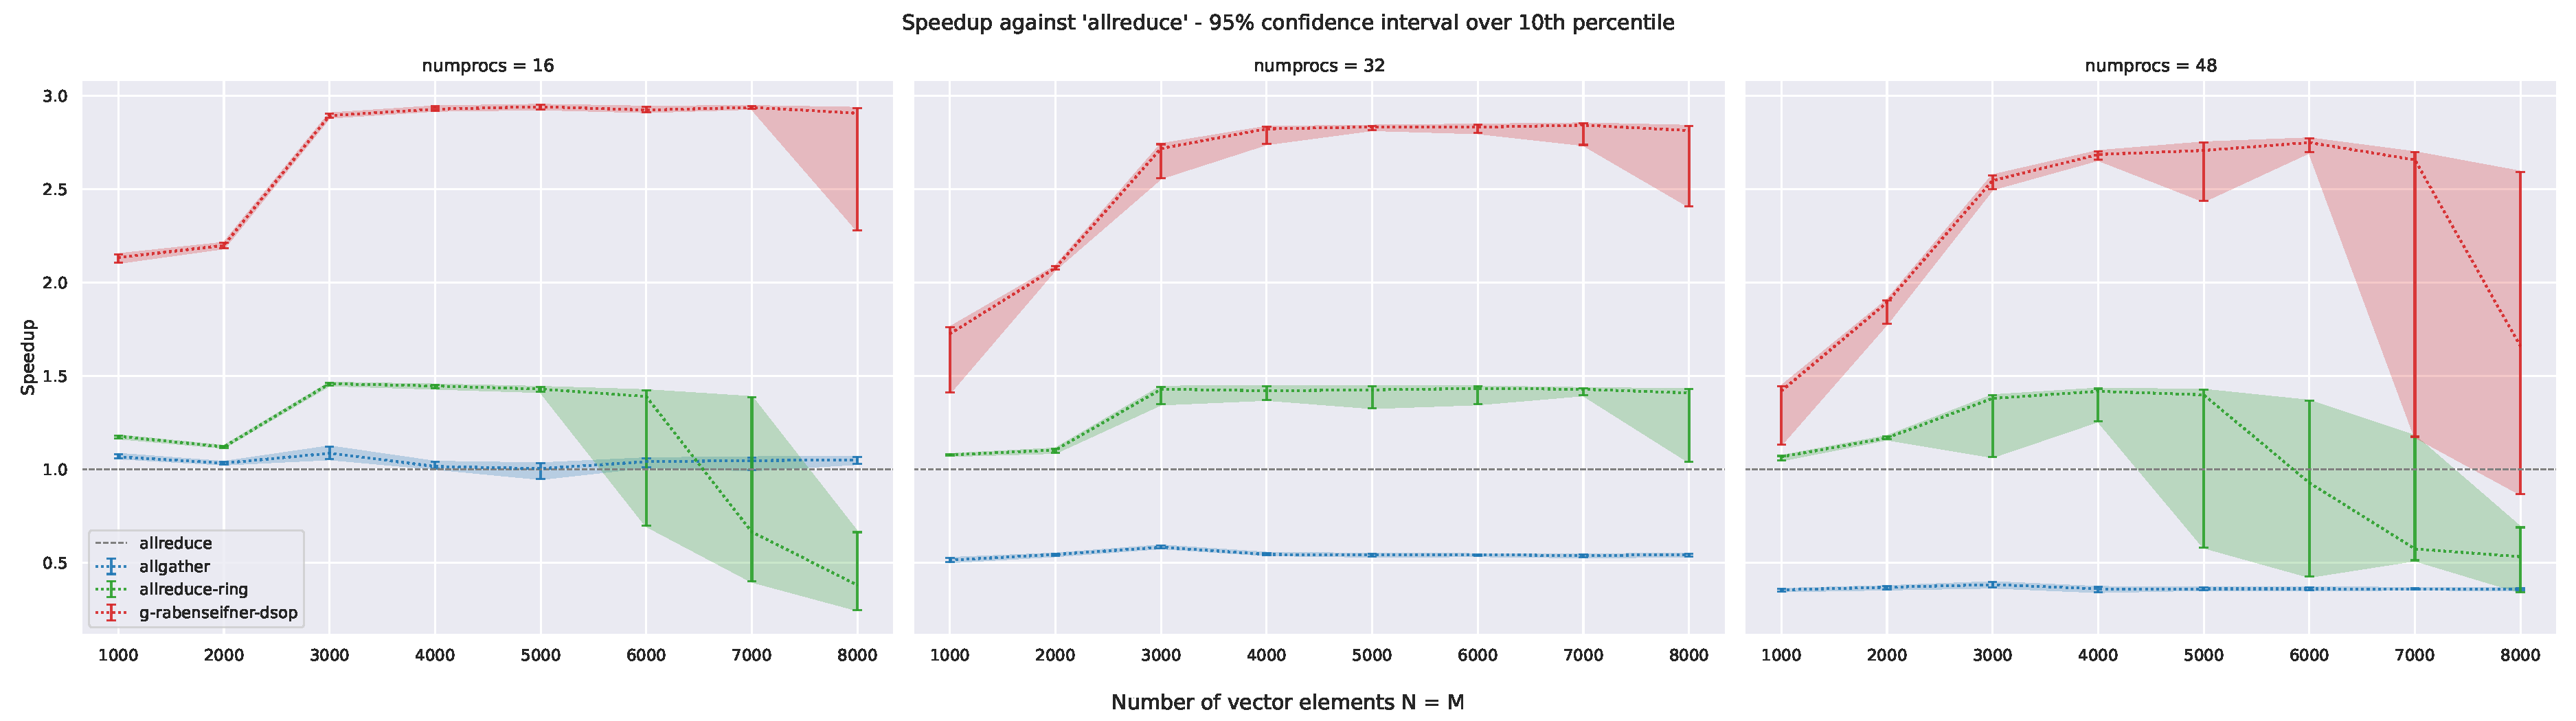
\includegraphics[width=\columnwidth]{plots/speedup_plot_N_numprocs_16_32_48__baseline_allreduce_percentile_10_CI_0.95_with_errorbar.pdf}
    \caption{10th percentile of speedups against base allreduce implementation with 95\% confidence interval, run with 16, 32, and 48 nodes}
\end{figure}

\begin{figure}[H]
    \centering
    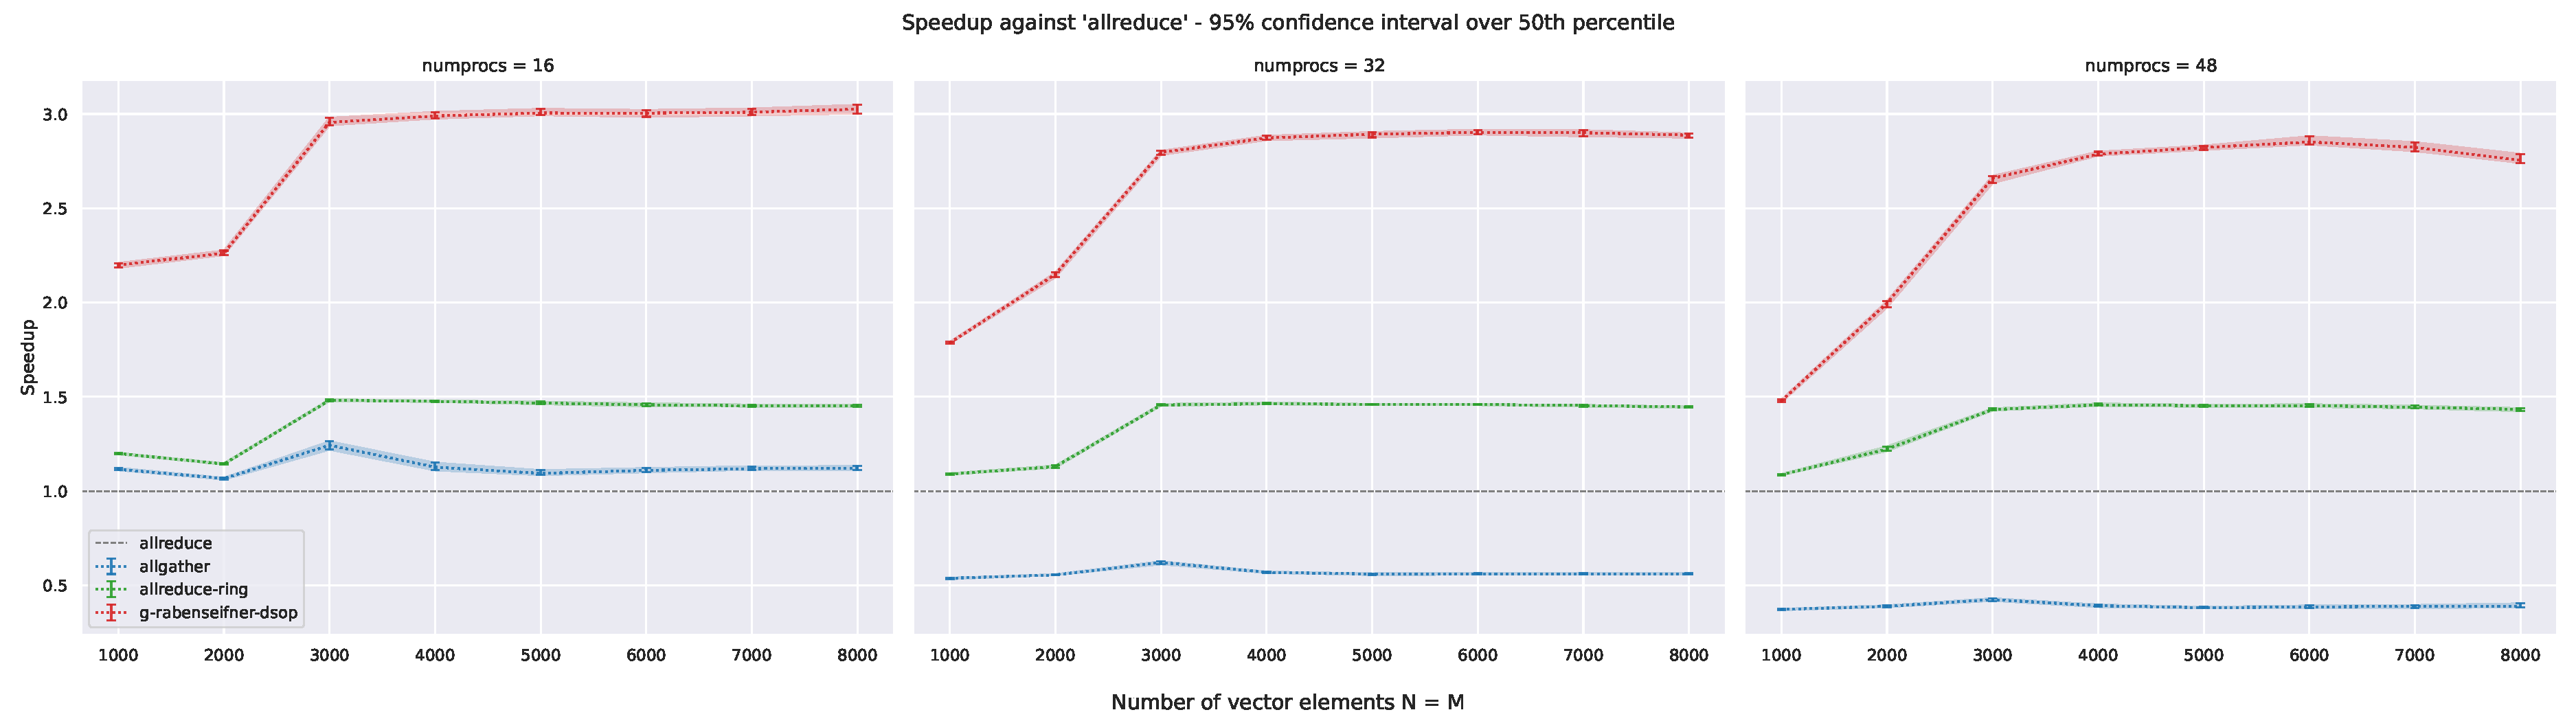
\includegraphics[width=\columnwidth]{plots/speedup_plot_N_numprocs_16_32_48__baseline_allreduce_percentile_50_CI_0.95_with_errorbar.pdf}
    \caption{Median speedup against base allreduce implementation with 95\% confidence interval, run with 16, 32, and 48 nodes}
\end{figure}

\begin{figure}[H]
    \centering
    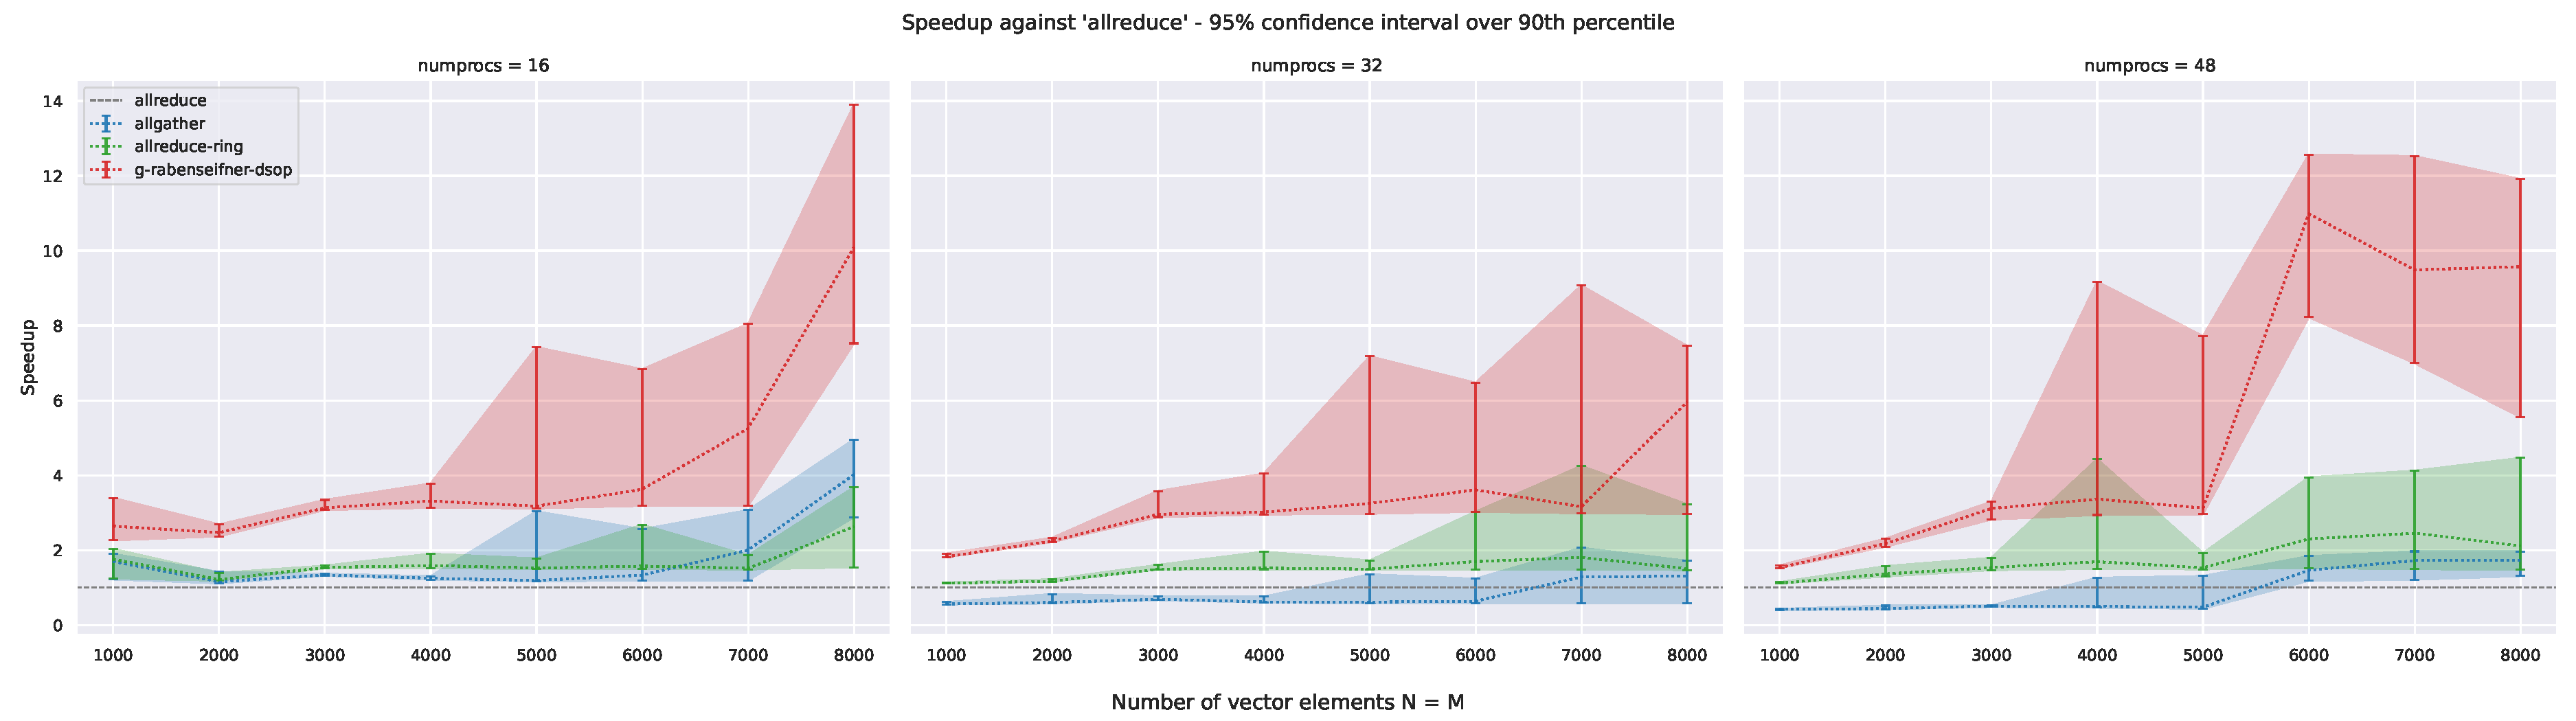
\includegraphics[width=\columnwidth]{plots/speedup_plot_N_numprocs_16_32_48__baseline_allreduce_percentile_90_CI_0.95_with_errorbar.pdf}
    \caption{90th percentile of speedups against base allreduce implementation with 95\% confidence interval, run with 16, 32, and 48 nodes}
\end{figure}

\subsection{Runtimes}

\begin{figure}[H]
    \centering
    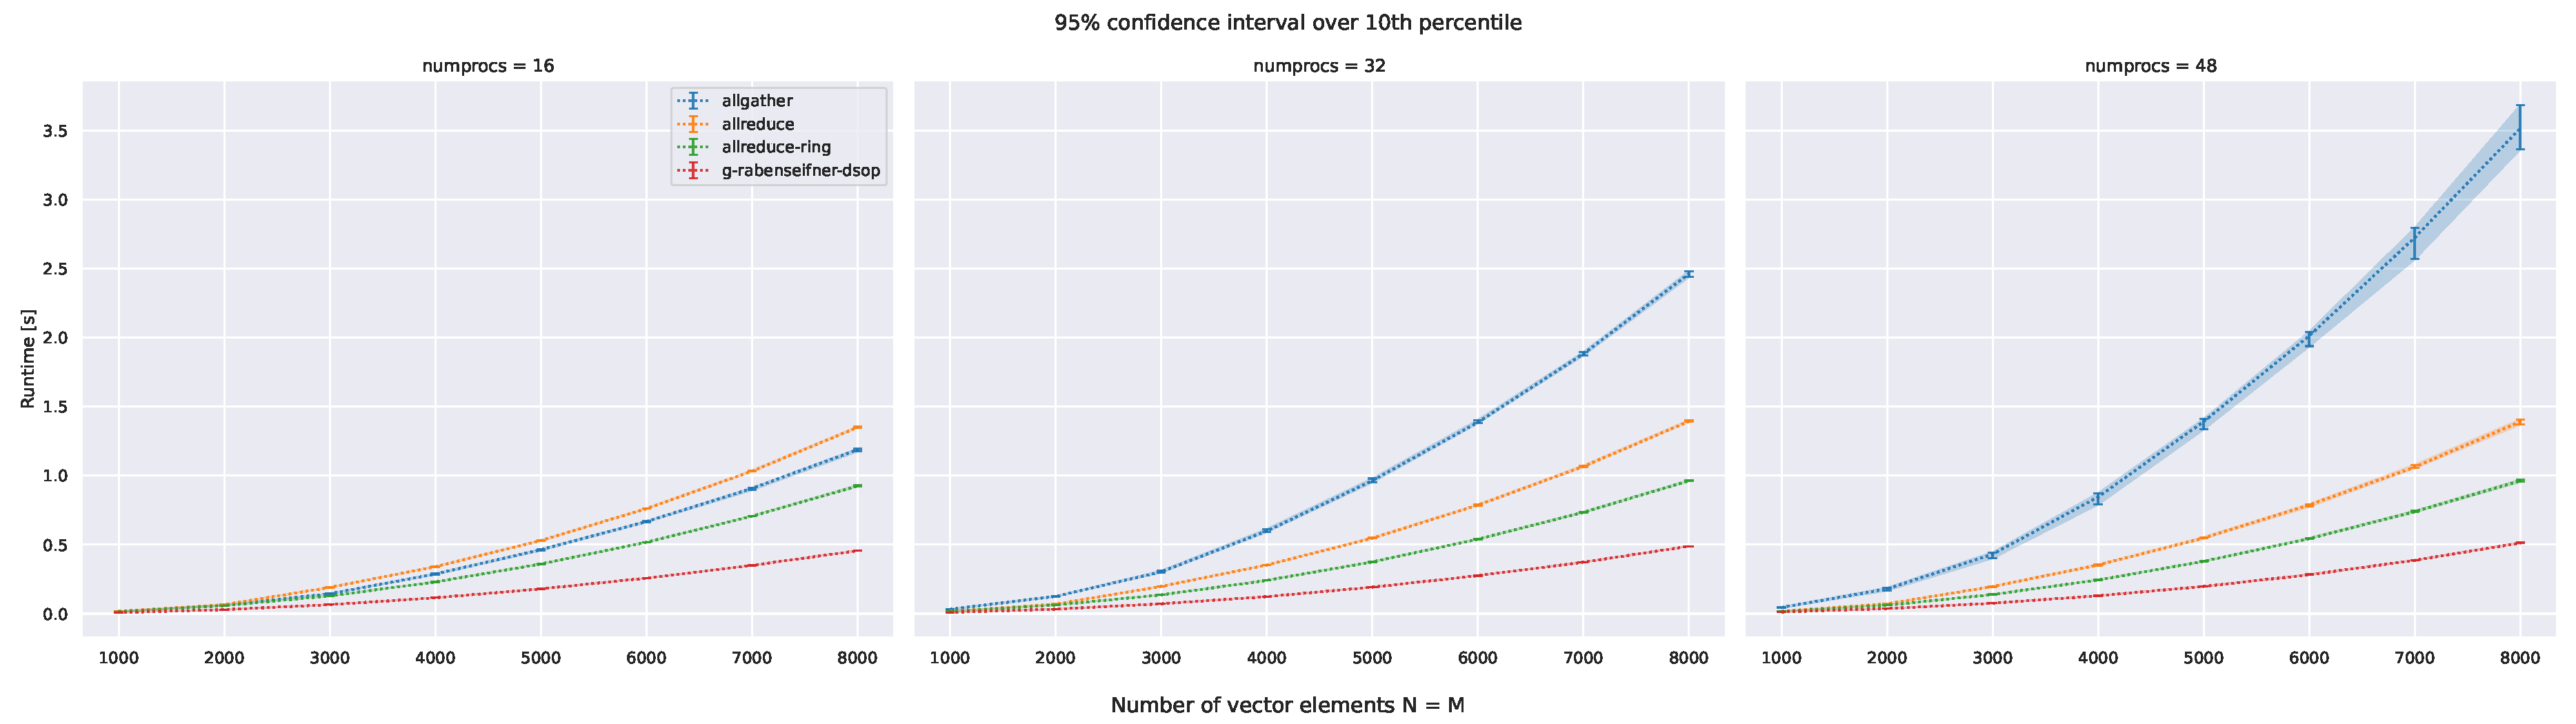
\includegraphics[width=\columnwidth]{plots/runtime_numprocs_16_32_48_N_percentile_10_CI_0.95_with_errorbar.pdf}
    \caption{10th percentile of runtimes with 95\% confidence interval, run with 16, 32, and 48 nodes}
\end{figure}

\begin{figure}[H]
    \centering
    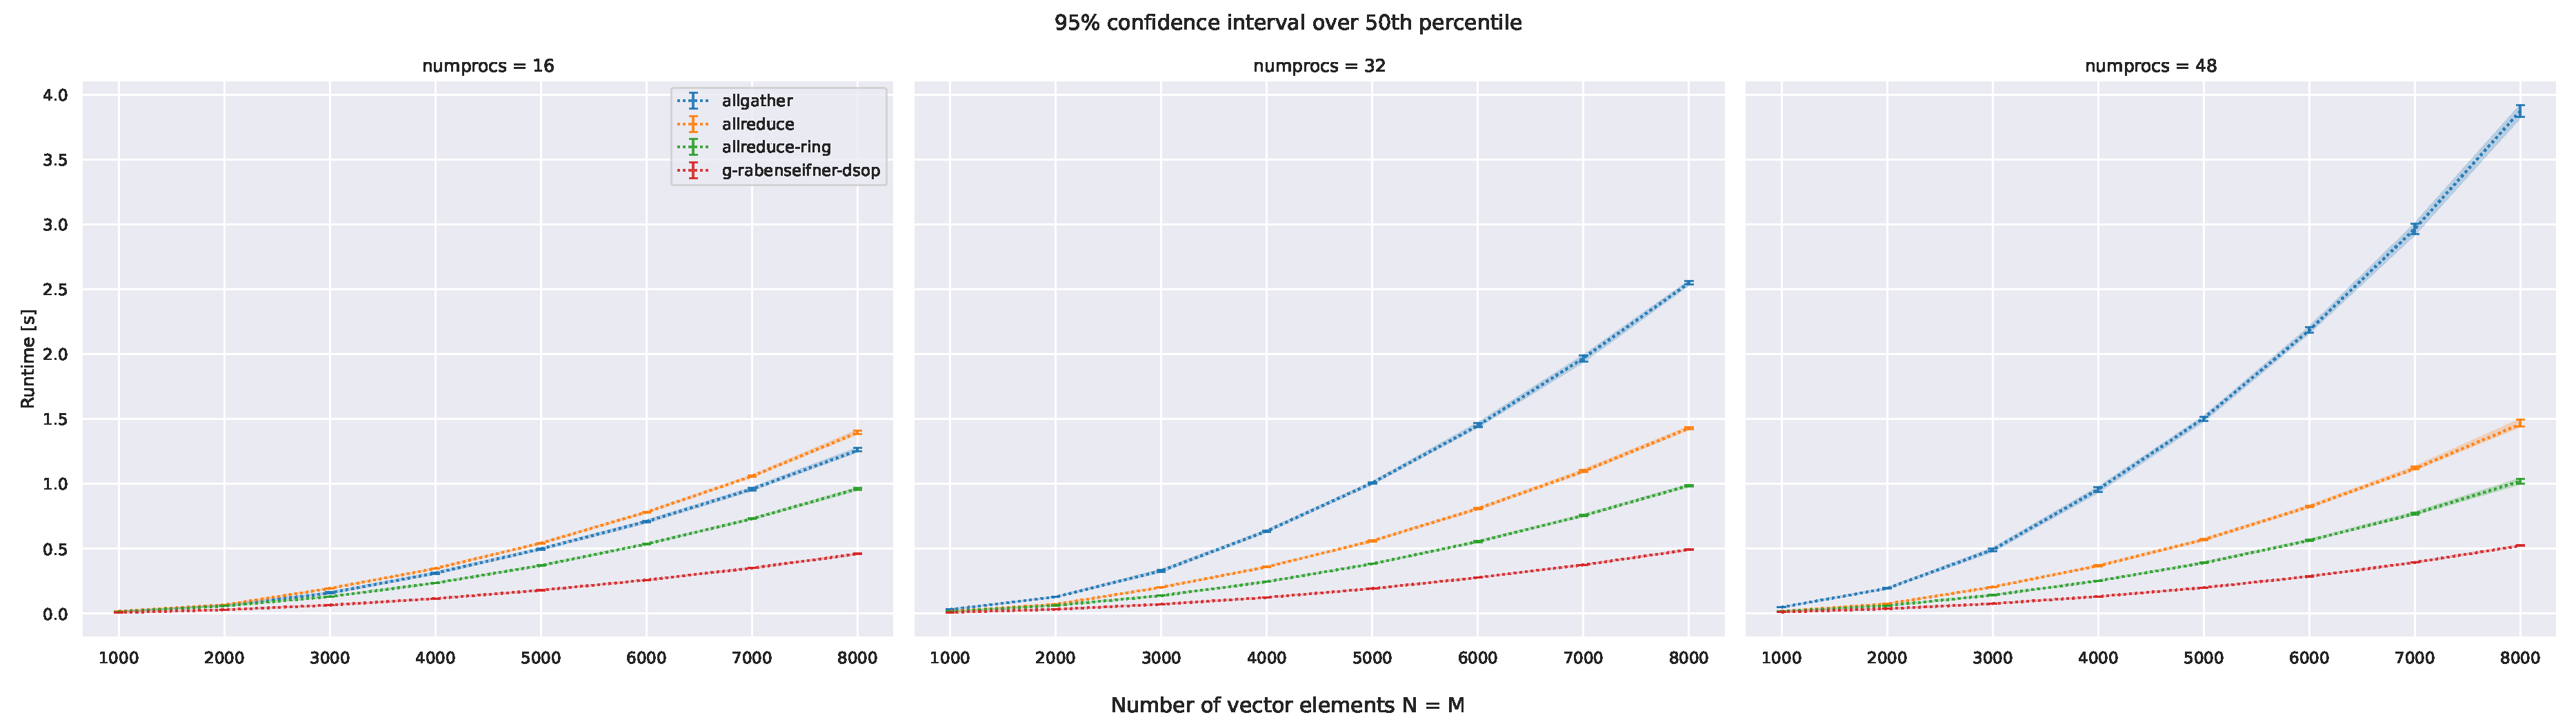
\includegraphics[width=\columnwidth]{plots/runtime_numprocs_16_32_48_N_percentile_50_CI_0.95_with_errorbar.pdf}
    \caption{Median runtimes with 95\% confidence interval, run with 16, 32, and 48 nodes}
\end{figure}

\begin{figure}[H]
    \centering
    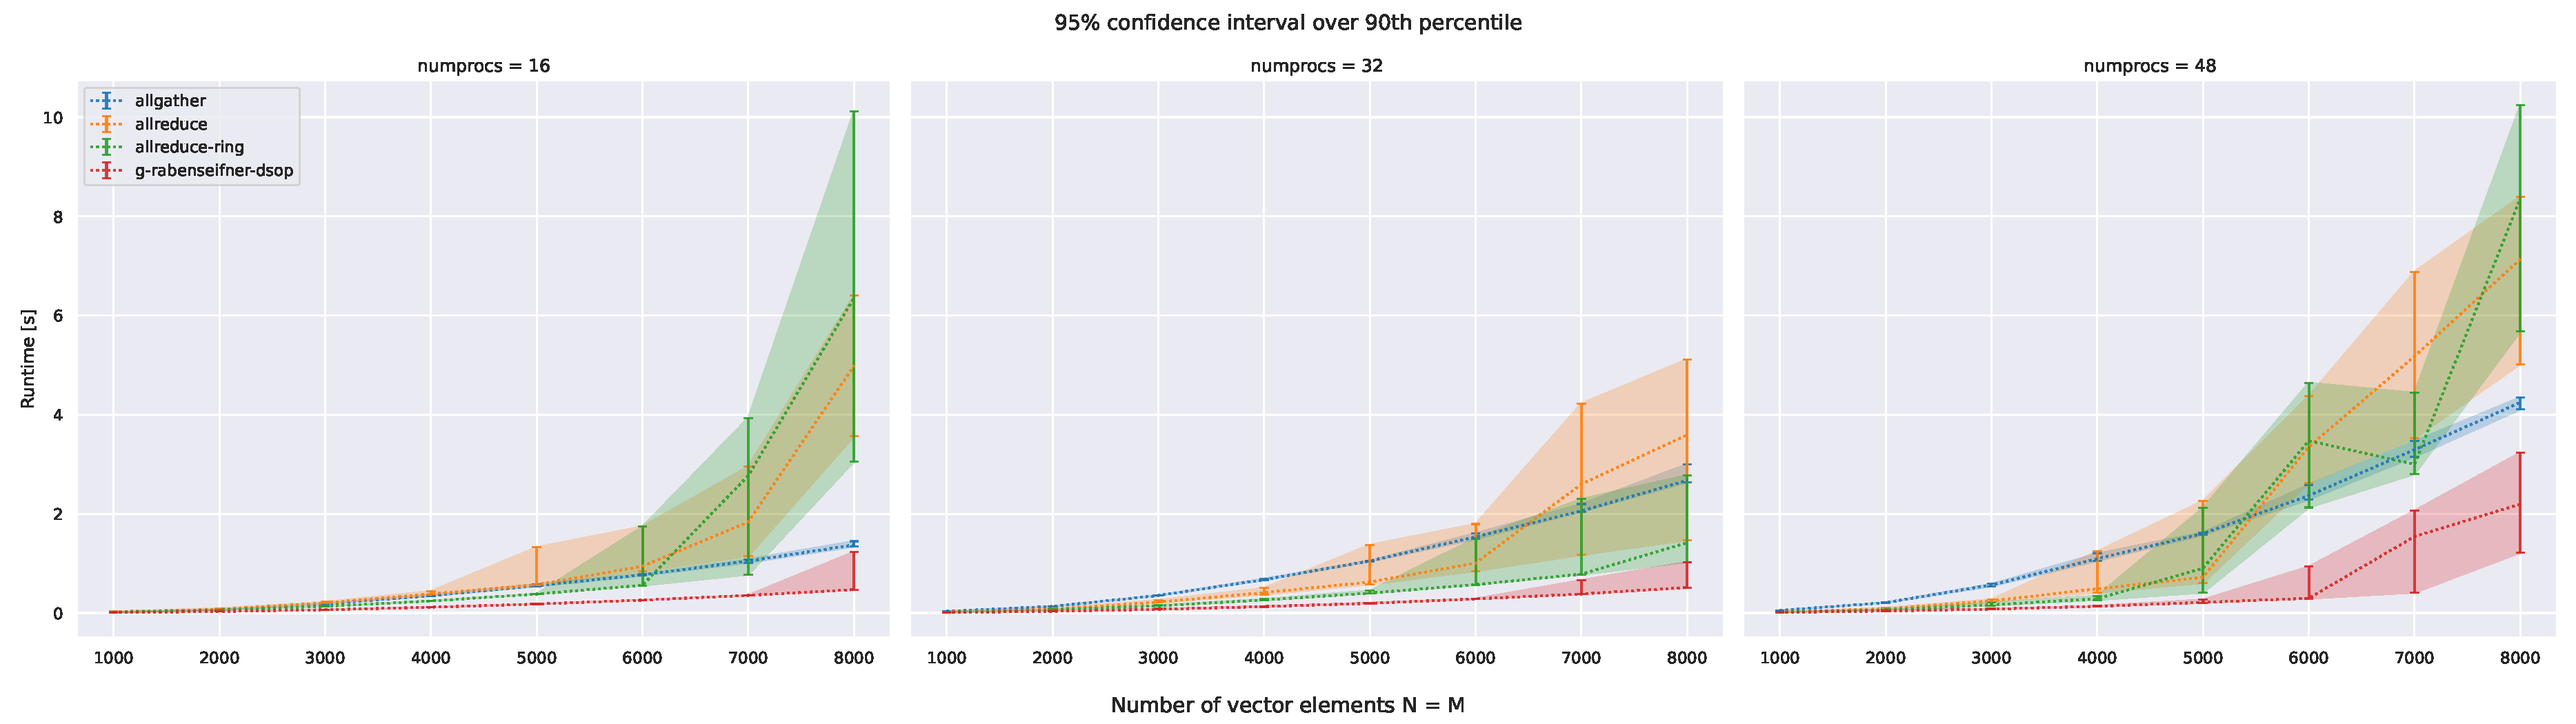
\includegraphics[width=\columnwidth]{plots/runtime_numprocs_16_32_48_N_percentile_90_CI_0.95_with_errorbar.pdf}
    \caption{90th percentile of runtimes with 95\% confidence interval, run with 16, 32, and 48 nodes}
\end{figure}

\subsection{Runtime Distributions}

\begin{figure}[H]
    \centering
    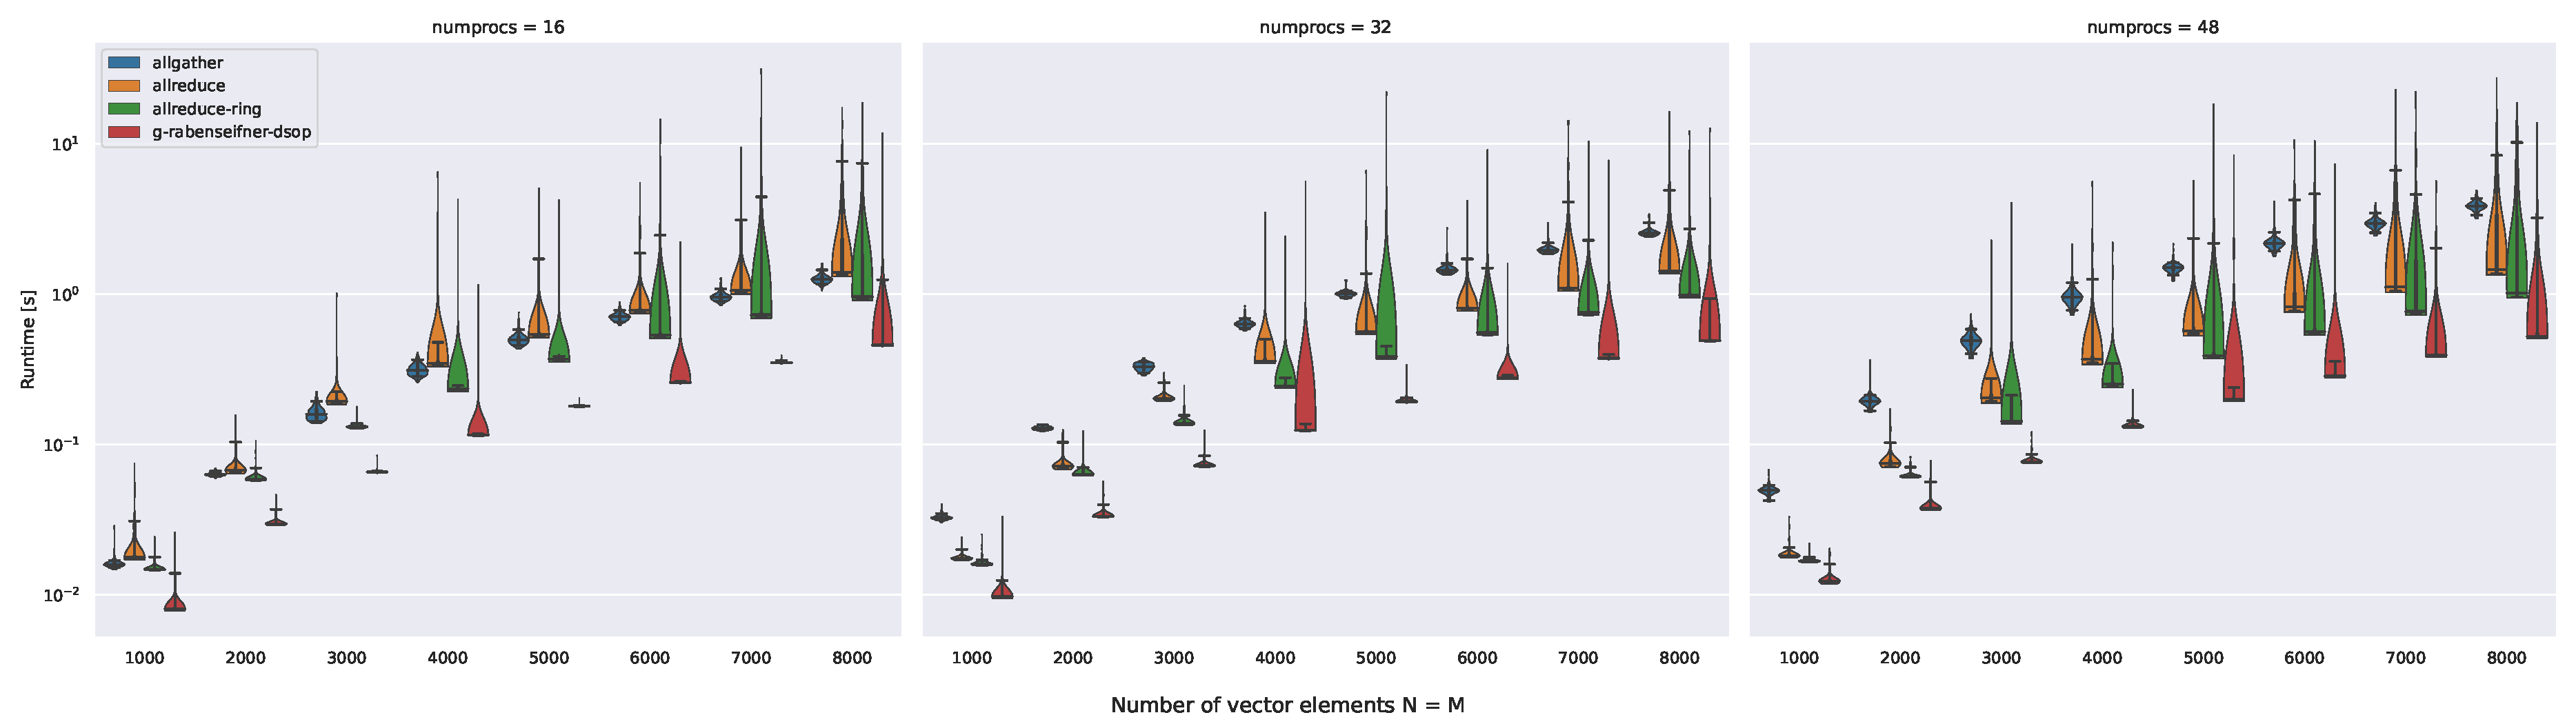
\includegraphics[width=\columnwidth]{plots/cmp_numprocs_16_32_48_log_scale.pdf}
    \caption{Runtime distributions per implementation on 16, 32, and 48 nodes.}
\end{figure}

\end{document}

